\documentclass[10pt]{article}

\usepackage[margin=0.75in]{geometry}
\usepackage{amsmath,amsthm,amssymb}
\usepackage{xcolor}
\usepackage{cancel}
\usepackage{graphicx}
\usepackage{changepage}
\usepackage{circuitikz}
\usepackage{pgfplots}
\usepackage{physics}
\usepackage{hyperref}
\usepackage{siunitx}
\usepackage[breakable]{tcolorbox}
\usepackage[inline]{enumitem}

\theoremstyle{definition}
\newtheorem{problem}{Problem}
\newtheorem{soln}{Solution}

\pgfplotsset{compat=newest}
\usetikzlibrary{lindenmayersystems}
\usetikzlibrary{arrows}
\usetikzlibrary{calc}

\definecolor{incolor}{HTML}{303F9F}
\definecolor{outcolor}{HTML}{D84315}
\definecolor{cellborder}{HTML}{CFCFCF}
\definecolor{cellbackground}{HTML}{F7F7F7}
\newcommand{\eq}{=}
\usetikzlibrary{positioning, fit, calc}
\pgfdeclarelayer{background}  
\pgfsetlayers{background,main}
\DeclareSIUnit[number-unit-product = {\,}]\calorie{cal}
\DeclareSIUnit[number-unit-product = {\,}]\atmosphere{atm}
\AtBeginDocument{\RenewCommandCopy\qty\SI}

\makeatletter
\newcommand{\boxspacing}{\kern\kvtcb@left@rule\kern\kvtcb@boxsep}
\makeatother
\newcommand{\prompt}[4]{
    \ttfamily\llap{{\color{#2}[#3]:\hspace{3pt}#4}}\vspace{-\baselineskip}
}

\newcommand{\thevenin}[2]{
  \begin{center}
    \begin{circuitikz} \draw
      (0,0) -- (2,0) to[battery1, l_=$V_{Th}\eq#1$] (2,2) 
      to[resistor, l_=$R_{Th}\eq#2$] (0,2)
      ;
      \draw [o-] (-.07,2.079);
      \draw [o-] (-.07,0.079);
    \end{circuitikz}
  \end{center}
}

\newcommand{\norton}[2]{
  \begin{center}
    \begin{circuitikz} \draw
      (0,0) -- (3,0) to[american current source, l_=$I_{N}\eq#1$] (3,2) -- (0,2) (2,0)
      to[resistor, l=$R_{N}\eq#2$] (2,2)
      ;
      \draw [o-] (-.07,2.079);
      \draw [o-] (-.07,0.079);
    \end{circuitikz}
  \end{center}
}

\newcommand{\highlight}[1]{\colorbox{yellow}{$\displaystyle #1$}}

\newcommand{\ti}[1]{\widetilde{#1}}

\title{Physics 2700H: Assignment III}
\author{Jeremy Favro (0805980) \\ Trent University, Peterborough, ON, Canada}
\date{\today}

\begin{document}
\maketitle

% PROBLEM 1
\begin{problem}
Five kg of water at $\qty{25}{\degreeCelsius}$ is added to $\qty{10.0}{\kilo\gram}$ of water at $\qty{85}{\degreeCelsius}$.
After the mixture has reached equilibrium, how much has entropy changed. (Assume no energy is exchanged between the water and its surroundings.)
\end{problem}
\begin{soln}
  The equilibrium temperature of the mixture can be determined using $Q=mc\Delta T$,
  \begin{align*}
    m_Cc\Delta T_C                      & =-m_Hc\Delta T_H                                           \\
    \implies m_C\left(T_f-T_{iC}\right) & =-m_H\left(T_f-T_{iH}\right)                               \\
    \implies T_f                        & =\frac{m_HT_{iH}+m_CT_{iC}}{m_C+m_H}=\qty{338.15}{\kelvin}
  \end{align*}
  Which means that $\Delta Q_C=836400=-Q_H$. To determine entropy change,
  \begin{align*}
    dS                & = \frac{dQ}{T}                   \\
    \implies \Delta S & =\int_{T_i}^{T_f}\frac{1}{T}\,dQ
  \end{align*}
  Where $Q=mc\Delta T\implies dQ=mcdT$ so
  \begin{align*}
    \Delta S & =mc\int_{T_i}^{T_f}\frac{1}{T}\,dT \\
             & =mc\ln\left(\frac{T_f}{T_i}\right)
  \end{align*}
  The entropy change of the system then is
  $\Delta S_{sys}=\Delta S_H +\Delta S_C=c\left[m_H\ln\left(\frac{T_f}{T_{iH}}\right)+m_C\ln\left(\frac{T_f}{T_{iC}}\right)\right]\approx \qty{229.46}{\joule\per\kelvin}$
  which is greater than zero as we would expect by the principle of increasing entropy.
\end{soln}
\newpage

% PROBLEM 2
\begin{problem}
The July 2023 Veritasium video about entropy, https://www.youtube.com/watch?v=DxL2HoqLbyA,
introduces a Carnot engine within the first six minutes of the video. Draw on a $PV$ diagram the cycle for
this engine, with the bottom-right-most point labelled (a), and continue the cycle to points (b), (c) and
(d). Identify which timestamps in the video correspond to the four points (a)… (d) and explain using a
sentence per point why this is so.
\end{problem}
\begin{soln}~
  % PV diagram - Carnot cycle
  \begin{center}
    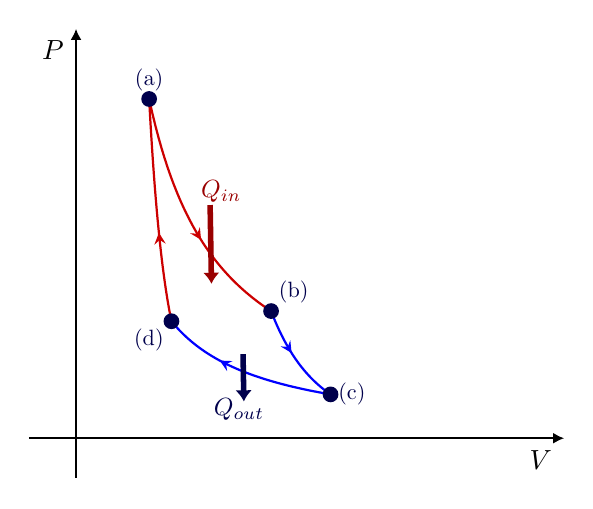
\begin{tikzpicture}[scale=2]
      \usetikzlibrary{arrows.meta} % to control arrow size
      \tikzset{>={Latex[length=4,width=4]}} % for LaTeX arrow head
      \usetikzlibrary{calc,decorations.markings,arrows.meta}
      \colorlet{mylightblue}{blue!20}
      \colorlet{myblue}{blue!80!black}
      \colorlet{mydarkblue}{blue!30!black}
      \colorlet{mylightred}{red!10}
      \colorlet{myred}{red!80!black}
      \colorlet{mydarkred}{red!60!black}
      \colorlet{mydarkgreen}{green!30!black}

      \def\N{40} % number of plot samples
      \def\xmax{3}
      \def\ymax{2.5}

      %\tikzstyle{midarr}=[decoration={markings,mark=at position 0.5 with {\arrow{stealth}}},postaction={decorate}]
      \tikzset{
        midarr/.style={decoration={markings,mark=at position #1 with {\arrow{stealth}}},postaction={decorate}},
        midarr/.default=0.5
      }

      \def\xtick#1#2{\draw[thick] (#1)++(0,.1) --++ (0,-.2) node[below=-.5pt,scale=0.9] {#2};}
      \def\ytick#1#2{\draw[thick] (#1)++(.1,0) --++ (-.2,0) node[left=-.5pt,scale=0.9] {#2};}


      \def\Th{1}
      \def\Tc{0.45}
      \def\Ch{0.1}
      \def\Cc{1.9}
      \def\N{40}
      \def\gam{4}
      \def\isotherm#1#2{{ #2/(#1) }}
      \def\adiabatic#1#2{{ #2/(#1)^(\gam) }}
      \def\xA{ (\Th/\Ch)^(1/(1-\gam)) }
      \def\xB{ (\Th/\Cc)^(1/(1-\gam)) }
      \def\xC{ (\Tc/\Cc)^(1/(1-\gam)) }
      \def\xD{ (\Tc/\Ch)^(1/(1-\gam)) }
      \coordinate (A) at ({\xA},{\isotherm{\xA}{\Th}});
      \coordinate (B) at ({\xB},{\isotherm{\xB}{\Th}});
      \coordinate (C) at ({\xC},{\isotherm{\xC}{\Tc}});
      \coordinate (D) at ({\xD},{\isotherm{\xD}{\Tc}});

      %\clip (-0.1*\xmax,-0.12*\ymax) rectangle (1.05*\xmax,1.1*\ymax);

      % % WORK
      % \fill[mylightblue,samples=\N]
      % plot[domain={\xA:\xB}] (\x,\isotherm{\x}{\Th}) --
      % plot[domain={\xB:\xC}] (\x,\adiabatic{\x}{\Cc}) --
      % plot[domain={\xC:\xD}] (\x,\isotherm{\x}{\Tc}) --
      % plot[domain={\xD:\xA}] (\x,\adiabatic{\x}{\Ch});
      % \node[blue,scale=.9] at ($(B)!.5!(D)$) {$W$};

      % ADIABATIC & ISOTHERMIC TRANSFORMATIONS
      \draw[myred,thick,midarr=.60,domain={\xA:\xB},samples=\N]
      plot (\x,\isotherm{\x}{\Th}); % hot
      \draw[blue,thick,midarr=.45,domain={\xB:\xC},samples=\N]
      plot (\x,\adiabatic{\x}{\Cc}); % cold
      \draw[blue,thick,midarr=.65,domain={\xC:\xD},samples=\N]
      plot (\x,\isotherm{\x}{\Tc}); % cold
      \draw[myred,thick,midarr=.40,domain={\xD:\xA},samples=\N]
      plot(\x,\adiabatic{\x}{\Ch}); % hot

      % POINTS
      \fill[mydarkblue]
      (A) circle(0.05) node[above,scale=.8] {(a)}
      (B) circle(0.05) node[above right,scale=.8] {(b)}
      (C) circle(0.05) node[right,scale=.8] {(c)}
      (D) circle(0.05) node[below left,scale=.8] {(d)};

      % HEAT
      \draw[>={LaTeX[width=6,length=4]},->,line width=2,mydarkred]
      ($(A)!.5!(B)$) --++ (-89:.5)
      node[pos=0,inner sep=0,anchor=-130,scale=.9] {$Q_{in}$};
      \draw[>={LaTeX[width=6,length=4]},->,line width=2,mydarkblue]
      ($(C)!.55!(D)$) --++ (-89:.3)
      node[inner sep=-2,anchor=60,scale=.9] {$Q_{out}$};

      % AXIS
      \draw[->,thick] (0,-0.1*\ymax) -- (0,\ymax+0.1)
      node[anchor=north east,inner sep=4,scale=1] {$P$};
      \draw[->,thick] (-0.1*\xmax,0) -- (\xmax+0.1,0)
      node[anchor=north east,inner sep=4,scale=1] {$V$};

    \end{tikzpicture}
    \begin{enumerate}[label=(\alph*)]
      \item 4:41 is when the hot block is brought into contact with the heat ``aperture'' and heat flows into the gas
            increasing temperature, pressure, and thereby driving an increase in volume.
      \item 4:53 the hot block is removed but the piston continues to climb and so volume increases and pressure decreases along an isotherm.
      \item 5:03 the cold block is brought into contact and the piston begins to move downwards with heat moving into the cold block, pressure increasing, and volume
            decreasing.
      \item 5:12 the cold block is removed and the has continues to be compressed, isothermally, meaning pressure increases and volume decreases.
    \end{enumerate}
  \end{center}
\end{soln}
\newpage

% PROBLEM 3
\begin{problem}
One mole of helium gas is initially at $P_0=\qty{1.0}{\atmosphere}$ and $T_0=\qty{273}{\kelvin}$.
\begin{enumerate}[label=(\alph*)]
  \item Compute the entropy change if the gas is heated at constant pressure to temperaturFe $\qty{400}{\kelvin}$.
  \item Starting again from the initial state $(P_0, T_0)$, what is the entropy change if
        the gas expands isothermally to twice its original volume?
\end{enumerate}
\end{problem}
\begin{soln}~
  \begin{enumerate}[label=(\alph*)]
    \item \begin{align*}
            \Delta S & = \int_{T_i}^{T_f}\frac{1}{T}\,dQ    \\
                     & = \int_{T_i}^{T_f}\frac{nC_P}{T}\,dT
          \end{align*}
          Where $C_P=C_V+nR$ where $C_V$ for an ideal monatomic gas is $\frac{3}{2}R$ so for one mole we have,
          \begin{align*}
            \Delta S & = \int_{T_i}^{T_f}\frac{\frac{5}{2}R}{T}\,dT                                \\
                     & = \frac{5}{2}R\ln\left(\frac{T_f}{T_i}\right)=\qty{7.94}{\joule\per\kelvin} \\
          \end{align*}
    \item Again,
          \begin{align*}
            \Delta S & = \int_{V_i}^{2V_i}\frac{1}{T}\,dQ
          \end{align*}
          Here we use the first law, $dU=dQ+dW$ where $dU$ is zero as $T$ is held constant and $dW=-PdV$ so $dQ=PdV$ so,
          \begin{align*}
            \Delta S & = \int_{V_i}^{2V_i}\frac{P}{T}\,dV                                      \\
                     & = \int_{V_i}^{2V_i}\frac{nR\cancel{T}}{V\cancel{T}}\,dV                 \\
                     & = \int_{V_i}^{2V_i}\frac{R}{V}\,dV                                      \\
                     & = R\ln\left(\frac{2V_i}{V_i}\right)\approx\qty{5.76}{\joule\per\kelvin} \\
          \end{align*}
  \end{enumerate}
\end{soln}
\end{document}